\chapter{Entropy}

\section{Entropy and entropy rate}
The definition of entropy of a random variable $X$ was originally given by Shannon in $1949$: Shannon stated that his main concern while studying such function was how to call it: luckily, while confronting his results wiht mathematician J. Von Neumann, he suggested that Shannon would call his function "Entropy", since, he stated:
\\"\textit{First: your function of uncertainty is already known in statistichal mechanics with that name; second and most of all, no one actually knows what entropy is, so you'll always have the upper hand in any discussion."}
\\Let $X$ be a random variable which takes values in the alphabet $\alp=\{ a_1, \dots, a_k \}$ with probabilities $\mu_j = \mathbb{P} (X=a_j)$. Then its entropy is defined as 
\begin{equation}
    \label{eq:entropy_def}
    H(X) \equiv -  \sum_{j=1}^k \mu_j \log \mu_j
\end{equation}
\\More generally, one could define Entropy as the expectation value of the information, which is defined as the logarithm of the probability mass function $p$:
\begin{equation*}
    H(X) = \mathbb{E}[I(X)] = \mathbb{E}[-\log p(X)]
\end{equation*}
The core idea of information theory is that the "informational value" of a communicated message depends on the degree to which the content of the message is surprising. If a highly likely event occurs, the message carries very little information. On the other hand, if a highly unlikely event occurs, the message is much more informative. 
\\For instance, the knowledge that some particular number will not be the winning number of a lottery provides very little information, because any particular chosen number will almost certainly not win. However, knowledge that a particular number will win a lottery has high informational value because it communicates the outcome of a very low probability event.
\\Entropy in information theory is directly analogous to the entropy in statistical thermodynamics. The analogy results when the values of the random variable designate energies of microstates, so Gibbs formula for the entropy is formally identical to Shannon's formula.

\subsection{Basic properties of the Entropy}
We now turn to look to some very basic but important properties of Entropy.
\\Let's be now more precise: consider a finite set $\mathcal{B} = \{ b_1, \dots, b_l \}$, so that $|\mathcal{B}| = L$, and let $\mathcal{P(\mathcal{B})} = \{ (p_1, \dots, p_l) : \sum_j p_j = 1, \, p_j \geq 0 \}$ be the set of all probability measures on $\mathcal{B}$ such that $p(b_k) = p_k$. Given $p \in \mathcal{P(\mathcal{B})} $ let's again define 
\begin{gather}
    \ent: \mathcal{P(\mathcal{B})} \longrightarrow \rb^+ \nonumber \\
    \ent(p) = - \sum_{b \in \mathcal{B}} p(b) \log p(b) = - \sum_{k=1}^l p_k \log p_k
\end{gather}
Such function satisfies the following conditions:
\begin{prop}[Entropy properties]
\label{prop:entropy_properties}
\hfill
\begin{itemize}
    \item[(1)]  $\bm{\ent(p) \geq 0}$ \textbf{and} $\bm{\ent(p) = 0}$ \textbf{iff} $\bm{p}$  \textbf{is pure}, i.e. $p$ is "concentrated" in one point, $p= (0,0, \dots, 0,1,0, \dots, 0)$. For example, a source emitting only one symbol with probability $1$.
    \item[(2)] $\bm{0 \leq \ent(p) \leq \log L}$. \\Specifically, $\ent(p) = \log L \Leftrightarrow p= (\frac{1}{L}, \dots, \frac{1}{L})$, i.e. when we have a sequence that is "maximally random" (a so called "chaotic sequence").
    \item[(3)] $\ent: \mathcal{P(\mathcal{B})} \longrightarrow [0, \log L]$ \textbf{is continous and concave}. 
    \\Concave meaning that if we take $p_1, \dots p_m \in \mathcal{P(\mathcal{B})}$ and consider a finite weighted linear combination $\alpha_1 p_1 + \dots + \alpha_m p_m$ where the weights satisfy $\sum_j \alpha_j = 1$, $\alpha_j \geq 0$, then
    \begin{gather}
        \label{eq:concavity_of_entropy}
        \ent (\alpha_1 p_1 + \dots + \alpha_m p_m) \geq \alpha_1 \ent (p_1) + \dots  \alpha_m \ent (p_m) \nonumber \, ,\\
        \ent (\alpha_1 p_1 + \dots + \alpha_m p_m) = \alpha_1 \ent (p_1) + \dots  \alpha_m \ent (p_m) \Leftrightarrow p_j=p_k \, \forall k
    \end{gather}
    
    \item[(4)] $\ent$ \textbf{is almost convex}, i.e. 
    \begin{equation}
        \ent (\alpha_1 p_1 + \dots + \alpha_m p_m) \leq \alpha_1 \ent (p_1) + \dots  \alpha_m \ent (p_m) + \ent (\alpha_1, \dots, \alpha_n)
    \end{equation}
    where $\ent (\alpha_1, \dots, \alpha_n) = - \sum_j \alpha_j \log \alpha_j$.
    Notice that $\alpha$ satisfies the properties of a measure, so that the weighted combination between $\alpha$ and $p$ can be looked at as a "mixture" of the two, meaning that when two measures "intersect" then their Entropy is no longer just additive.
\end{itemize}
\end{prop}
Recall that a function $f(x)$ is said to be convex over the interval $(a, b)$ if $\forall x_1, x_2 \in (a, b)$ and $0 \leq \lambda \leq 1$:
\begin{equation*}
    f(\lambda x_1 + (1 - \lambda)x_2) \leq \lambda f(x_1) + (1- \lambda) f(x_2)
\end{equation*}
The function $f$ is strictly convex if the equality holds only if $\lambda=0$ or $\lambda=1$. Also, recall that (this can be prove by Taylor expansion of $f$) if the function f has a second derivative that is non-negative (positive) over
an interval, the function is convex (strictly convex) over that interval.
\\Let's now prove the proposition \ref{prop:entropy_properties}.
\begin{proof}
\hfill
    \begin{itemize}
        \item[(2)] follows from the Jensen Inequality (stated below)
        \item[(1),(3)] follow from the fact that $f(x) = -  x\log x = 0 \Leftrightarrow x=0$ or $x=1$
        \item[(4)] 
        \begin{align*}
            \ent (\alpha_1 \mu_1 + \dots + \alpha_d \mu_d) = & \sum_{k=1}^d \sum_{b \in \mathcal{B}} - \alpha_k \mu_k(b) \log \big( \sum_{j=1}^d \alpha_j \mu_j (b)  \big) \leq  \\ & \leq \sum_{k=1}^d \sum_{b \in \mathcal{B}} - \alpha_k \mu_k(b) \log (\alpha_k \mu_k (b)) = \\ & = \sum_{k=1}^d \sum_{b \in \mathcal{B}} - \alpha_k \mu_k(b) \log \alpha_k - \alpha_k \mu_k(b) \log \alpha_k = \\ & = \sum_{k=1}^d \alpha_k \ent (\mu_k) + \ent(\alpha_1 \mu_1, \dots, \alpha_d)
        \end{align*}
        where the first inequality is trivial due to the monotonicity of the logarithm.
    \end{itemize}
\end{proof}

\begin{theorem}[Jensen Inequality]
\label{th:jensen_inequality}
            Let $f: \rb \rightarrow \rb$ be convex. Then if we consider any finite set $\{ \alpha_j \}$ such that $\sum_{j=1}^d \alpha_j = 1$ we have that
            \begin{equation*}
                f(\alpha_1 x_1 + \dots + \alpha_d x_d) \geq \sum_{j=1}^d \alpha_j f(x_d)
            \end{equation*}
            In the context of probability theory, it is generally stated in the following form: 
            \\If $f$ is a convex function and $X$ is a random variable, then 
            \begin{equation}
                \mathbb{E}\big[ f(X) \big] \geq f \big( \mathbb{E}\big[X\big] \big)
            \end{equation}
\end{theorem}
We will prove this in a simple setting, i.e. for atomic measures.
\begin{proof}
\hfill
    For a two-mass-point distribution, directly from the definition of convex function we have 
    \begin{equation*}
        p_1 f(x_1) + p_2 f(x_2) \geq f (p_1 x_1 + p_2 x_2)
    \end{equation*}
    So the Jensen inequality is true in this case. Now we use induction. Suppose the theorem being true for $k-1$ atoms. Writing $p'_1 = p_i/1-p_k$ for $i = 1,2, \dots, k-1$:
    \begin{align*}
        \sum_{i=1}^k p_i f(x_i) & = p_k f(x_k) + (1 - p_k) \sum_{i=1}^{k-1} p_i' f(x_i) \geq \\ & \geq p_k f(x_k) + (1-p_k) f \big( \sum_{i=1}^{k-1} p_i' f(x_i) \big) \geq \\ & \geq f \big( p_k x_k + (1-p_k) \sum_{i=1}^{k-1} p_i' f(x_i) \big) = \\ & = f ( \sum_{i=1}^k p_i x_i )
    \end{align*}
\end{proof}

 \subsection{n-block Entropy}
 \label{par:n_block_entropy}
Let's now generalize to the case where $\mathcal{B} = \alp^n$. We define the $n-$block entropy of a stochastic process as 
\begin{equation}
    \label{eq:n_block_entropy}
    H_n(\mu) \equiv - \sum_{\omega_1^n \in \alp^n} \mu(\omega) \log \mu(\omega) 
\end{equation}
which we sometime denote equivalently as $H_n(\omega_1^n) = H(\omega_1, \dots, \omega_n)$. 
\\Let now $\alp$ be separable in the cartesian product of two alphabets, $\alp^n = \alp^l \times \alp^r$, with $l+r=n$. Let's then denote $b \in \alp^n$ as $b=(a^l, a^r)$ with $a^l \in \alp^l$ and $a^r \in \alp^r$.
\\Consider now $\mu: \alp^n \rightarrow [0, 1]$. We know of course that 
\begin{equation*}
    \sum_{b \in \alp^n} \mu(b) = \sum_{a^l \in \alp^l, a^r \in \alp^r} \mu(a^l, a^r) = 1
\end{equation*}
and that we can define the marginals 
\begin{gather*}
    \mu_l (\cdot) = \sum_{a^r \in \alp^r} \mu(\cdot, a^r) \\
    \mu_r (\cdot) = \sum_{a^l \in \alp^l} \mu(a^l, \cdot)
\end{gather*}
Given now a word $\omega \in \text{supp}\, \mu_l = \{ b \in \alp | \mu_l(b) > 0 \}$ we can define the \textbf{conditional} $\forall \omega' \in \alp^r$
\begin{equation}
    \mu^{\omega}_{r|l} (\omega') = \frac{\mu(\omega, \omega')}{\mu_l(\omega)}
\end{equation}
or equivalently 
\begin{equation}
    \mu(\omega, \omega') = \mu_l(\omega) \cdot \mu^{\omega}_{r|l} (\omega')
\end{equation}
Now in this setup, if we consider again the Entropy $\ent : \mathcal{P}(\mathcal{B}) \rightarrow [0, \log L]$ with $|\alp^n| = L$, we can prove that 
\begin{prop}[Conditional Entropy]
\hfill
    \begin{itemize}
        \item[(a)] $\ent (\mu) = \ent(\mu_l) + \sum_{\omega \in \alp^l} \mu_l(\omega) \ent (\mu^{\omega}_{r|l})$ 
        \\\\i.e., the Entropy of the whole system is given by the entropy of the subsystem $+$ conditional entropy, weighted on $\mu_l(\omega)$
        \item[(b)] $\ent(\mu) \leq \ent(\mu_l) + \ent(\mu_r)$;
        \\ $\ent(\mu) = \ent(\mu_l) + \ent(\mu_r) \Leftrightarrow \mu = \mu_l \otimes \mu_r$
    \end{itemize}
\end{prop}
This definition also for $n-$block entropy, namely it is connected to the definition of the Entropy rate:
\begin{definition}[Entropy rate and n-conditional Entropy]
    \begin{equation}
        h_n(\mu) \equiv H_{n+1}(\mu) - H_n(\mu) = - \sum_{\omega_1^n \in \alp^n, a \in \alp} \mu(\omega_1^n a) \log \mu (a | \omega_1^n)
    \end{equation}
\end{definition}
Such object can be given the interpretation of information that we get by knowing a new character (adding a character to our sequence). 
But what exactly is $H_{n+1}$? How come that conditional Entropy gets in the picture? We can actually directly compute $H_{n+1}$: consider a decomposition $\alp^{n+1} = \alp^n \times \alp$ so that $(\omega_1 \dots \omega_{n+1}) \equiv (\omega_1^n, \omega_{n+1})$. Then,
\begin{align*}
    H_{n+1} = & - \sum_{\omega_1 \dots \omega_n, \omega_{n+1}} \log \mu(\omega_1 \dots \omega_n \omega_{n+1}) = \\ &=  - \sum_{\omega_1^n \in \alp^n, \omega_{n+1} \in \alp} \mu (\omega_1^n, \omega_{n+1}) \log \big( \mu(\omega_1^n) \mu(\omega_{n+1} | \omega_1^n) \big) = \\ & =  - \sum_{\omega_1^n \in \alp^n, \omega_{n+1} \in \alp} \mu (\omega_1^n, \omega_{n+1}) \big\{ \log \mu(\omega_1^n) + \log \mu(\omega_{n+1} | \omega_1^n) \big\} 
\end{align*}
Now, since we can first sum on the last character and we know that $\sum_{\omega_{n+1} \in \alp} \mu(\omega_1, \dots, \omega_n, \omega_{n+1}) = \mu_n(\omega_1, \dots, \omega_n)$, we finally get 
\begin{equation*}
    H_{n+1} = H_n - \sum_{\omega_1^n \in \alp^n, \omega_{n+1} \in \alp} \mu(\omega_1^n \omega_{n+1}) \log \mu (\omega_{n+1} | \omega_1^n)
\end{equation*}
We can also generalize this result to the case of $H_{n+m}$: consider $\alp^{n+m} = \alp^n \times \alp^m$ and $(\omega_1, \dots, \omega_{n+m}) \equiv (\omega^1 \in \alp^n, \omega_2 \in \alp^m)$. Then
\begin{align*}
    H_{n+m} = & - \sum_{\omega^1 \in \alp^n, \omega_2 \in \alp^m} \mu(\omega^1, \omega^2) \log \mu(\omega^1, \omega^2) = \\ & = - \sum_{\omega^1 \in \alp^n, \omega_2 \in \alp^m} \mu(\omega^1, \omega^2) \big( \log \mu(\omega^1) + \log \mu(\omega^2 | \omega^1) \big) = \dots  =\\ & = H_n (\mu) - \sum_{\omega^1 \in \alp^n} \mu(\omega^1) H_m (\mu^{\omega^1} (\cdot))
\end{align*}
where the first passage comes from the fact that $\mu(\omega^1, \omega^2) = \mu(\omega^1) \mu(\omega^2 | \omega^1)$ and $\mu^{\omega^1} (\cdot)$ is the conditional entropy to $\omega^1$ as introduced before.\\
\textit{exercise: finish the demonstration}
\\Also, if we have $\mu: \alp^{n+1} \rightarrow \rb$ and a function $f: \alp^{n+1} \rightarrow \rb$ we can define very naturally the expectation value of $f$,
\begin{equation*}
    \mathbb{E}_{\mu_{n+1}} [f] \equiv \sum_{\omega_1 \dots \omega_{n+1} \in \alp} \mu(\omega_1 \dots \omega_{n+1}) f(\omega_1 \dots \omega_{n+1})
\end{equation*}
In this way we also get 
\begin{equation*}
    h_n(\mu) = \mathbb{E}_{\mu_{n+1}} [ \log \mu(a|\omega_1^n)]
\end{equation*}
After the definition of the Entropy rate, we can define the "Entropy per character" $\frac{H_n(\mu)}{n}$ \footnote{notice that $0 \leq H_n(\mu) \leq \log |\alp^n| = \log|\alp|^n$ so that $\frac{H_n(\mu)}{n} \leq \log |\alp|$}.
\\We then define the Entropy of the source $\mu$ to be 
\begin{definition}
    \begin{equation}
    \label{eq:h(mu)_definition}
        h(\mu) = \lim_{n \rightarrow \infty} \frac{H_n(\mu)}{n} =  \lim_{n \rightarrow \infty} h_n(\mu) = \mathbb{E}_{\mu} (\log \mu(a | \omega_1^{\infty}))
    \end{equation}
\end{definition}
where the last expression denotes the average value of "infinite information", as if we knew all of the history of the system (future and past), i.e. as if we had an infinite data sample. 
\\The existence of the limit (\ref{eq:h(mu)_definition}) is guaranteed by the subadditivity lemma: 
\begin{lemma}[subadditivity lemma]
\hfill
    If $\{ x_n \}$ is a sequence of nonnegative numbers, which is subadditice, i.e. 
    \begin{equation*}
        x_{n+m} \leq x_n + x_m
    \end{equation*}
    then 
    \begin{equation*}
        \lim_{n \rightarrow \infty} \frac{x_n}{n} = \liminf_{n \rightarrow \infty}\frac{x_n}{n}
    \end{equation*}
\end{lemma}
\begin{proof}
    Left as an exercise
\end{proof}
Notice that since $h_k = H_{k+1} - H_k$ we have that
\begin{equation*}
    h(\mu) \leq \dots h_k(\mu) \leq h_{k-1}(\mu) \leq \dots \leq h_1(\mu) \leq H_1(\mu)
\end{equation*}
\textit{exercise:} prove it

\subsubsection{Two classical and easy examples}
Let $X$ be a i.i.d. process, with $\mu_k = \mathbb{P}(X_j = a_k)$, $k = 1, \dots, |\alp|$. 
\\Then we have that 
\begin{equation}
    h(X) = \lim_{n \rightarrow \infty} \frac{n H(X_j)}{n} = H(X_j)
\end{equation}
i.e., the entropy of the process is equal to the entropy of any of its variables.
\\Let $X$ be a stationary $k-$Markov: the Markov property $\mu(\omega_{n+1}| \omega_1 \dots \omega_n) = \mu(\omega_{n+1}| \omega_{n-k+1} \dots \omega_n)$ ensures that 
\begin{equation}
\label{eq:markov_entropy}
    h_n = h_k \quad \forall n \geq k
\end{equation}
i.e., the entropy stabilises to a certain value. Since this is an if and only if, \textbf{we can also infer if a system is $k$-Markov if $h_n$ stabilises to a certain value. } We will see the proof of this statement later on (see \cref{par:mutual_information}).

\section{Cross and Relative entropy}
In this section we focus on properties involving pairs of stochastic sources
on the same alphabet with distributions  $\mu$ and $\nu$: the \textbf{\textit{cross entropy}} and the related \textbf{\textit{relative entropy}} (or \textbf{\textit{Kullback-Leibler divergence}})
\\Firs, let's define the $n-$conditional cross entropy as
\begin{equation}
    h_n(\mu || \nu) = - \sum_{\omega \in \alp^n, a \in \alp} \mu(\omega a) \log \nu(a| \omega)
\end{equation}
and then we define
\begin{definition}[cross entropy]
    \begin{equation}
        h(\mu || \nu) = \lim_{n \rightarrow \infty} h_n(\mu || \nu)
    \end{equation}
\end{definition}
and moreover we define 
\begin{definition}[relative entropy (Kullback-Leibler divergence)]
    \begin{align}
        d(\mu || \nu) = \lim_{n \rightarrow \infty} \mathbb{E} \bigg[ \log \frac{\mu(\omega_n|\omega_1^{n-1})}{\nu(\omega_n|\omega_1^{n-1})} \bigg] = \\ = \lim_{n \rightarrow \infty} \sum_{\omega_1^n \in \alp^n} \mu(\omega_1^n) \log \frac{\mu(\omega_n|\omega_1^{n-1})}{\nu(\omega_n|\omega_1^{n-1})}
    \end{align}
\end{definition}
The Kullback-Leibler divergence is not symmetric, but can easily be symmetrized by defining
\begin{equation}
    \Delta(\mu, \nu) = \frac{1}{2} d(\mu || \nu) +  \frac{1}{2} d(\nu || \mu) 
\end{equation}
Now, such function is symmetric and it can be proven (as we will see later on) to be positive, i.e. $\Delta=0 \Leftrightarrow \mu = \nu$ and $\Delta \geq 0$. Therefore it \textit{looks like a distance}, even though it doesn't satisfy the triangular inequality. 
\\The relative entropy is a measure of the distance between two distributions. In statistics, it arises as an expected logarithm of the likelihood ratio.
The relative entropy $d(p||q)$ is a measure of the inefficiency of assuming
that the distribution is $q$ when the true distribution is $p$. For example, if we knew the true distribution $p$ of the random variable, we could construct a code with average description length $H (p)$. If, instead, we used
the code for a distribution $q$, we would need $H (p) + d(p||q)$ bits on the
average to describe the random variable.
\\Entropy and cross entropy can be related to the asymptotic behavior of properly defined \textit{returning times} and \textit{waiting times}, respectively, which are two mathematical objects widely used in applications. 
\begin{definition}[Returning time]
    \hfill
    I read the first $n-$word and ask myself how much time I have to wait until I see again such sequence:
    \begin{equation}
        R(\omega_1^n) = \min{k>1: \omega_k^{k+n-1} = \omega_1^n}
    \end{equation}
\end{definition}
This object is purely combinatoric, it depends only on the sequence and not on the probability of seeing the sequence: but as we'll see, it can give information on the source itself. 
\\If $\omega$ is emitted by an ergodic source, such time exists and is finite\footnote{Poincaré Recurrence Theorem}. 
Supposing now to have two sources which emit two sequences $z \in \mu$ and $\omega \in \nu$. We can define
\begin{definition}[Waiting time]
    \hfill
    I read the first $n-$word in the sequence $\omega$ and ask myself how much time I have to wait until I see again such sequence in the other sequence $z$:
    \begin{equation}
        W(\omega_1^n, z) = \min{k>1: z_k^{k+n-1} = \omega_1^n}
    \end{equation}
\end{definition}
Note that $W(\omega_1^n, \omega) = R(\omega_1^n)$.
\\There are two important results which we are not going to prove about such times we defined above: 
\begin{theorem}[Entropy and returning time]
If $\mu$ is a stationary and ergodic process, then 
\begin{equation}
    \lim_{n \rightarrow \infty} \frac{1}{n} \log R(\omega_1^n) = h(\mu) \quad \mu-\text{a.s.}
\end{equation}
\end{theorem}
This connects our data with the source. Again, $R$ is a purely topological quantity, combinatorial, unrelated in principle to the source; but if we assume that the sequence $\omega$ is typical with respect to the source $\mu$, then $R$ converges to the Entropy. This is a very deep result which we can proved starting from the SMB Theorem (see \ref{th:SMB}). 
\\Moreover, we have that
\begin{theorem}[Relative entropy and waiting time]
If $\mu$ is a stationary and ergodic process, $\nu$ is $k-$Markov and $\mu_n << \nu_n$, then 
\begin{equation}
    \lim_{n \rightarrow \infty}  \log W(\omega_1^n, z) = h(\mu) + d(\mu || \nu) = h(\mu || \nu) \quad \mu \times \nu-\text{a.s.}
\end{equation}
\end{theorem}
In relation with the Kullback-Liebler we have, thanks to the Jensen Inequality \ref{th:jensen_inequality}, an important result:
\begin{theorem}[Information inequality]
    For any couple of probability distributions $\mu$ and $\nu$ for which $d(\mu || \nu)$ is defined,
    \begin{equation}
        d(\mu || \nu) \geq 0
    \end{equation}
    and the equality holds iff $\nu = \mu$.
\end{theorem}
\begin{proof}
    Let $A = x : p(x) > 0$ be the support of $p(x)$. Then
    \begin{align*}
        - d (\mu || \nu) & = \\
        & = \sum_{a \in A} \mu(a) \log \frac{\mu(a)}{\nu(a)} = \\ 
        & =  \sum_{a \in A} \mu(a) \log \frac{\nu(a)}{\mu(a)} \leq \\
        & \leq \log \big( \sum_{a \in A} \mu(a) \frac{\nu(a)}{\mu(a)} \big) = \\ 
        & = \log \big( \sum_{a \in A} \nu(a \big) = \log 1 = 0
    \end{align*}
\end{proof}

\section{Mutual information}
\label{par:mutual_information}
Let's now consider a pair of discrete random variables $(x, y)$ with joint distribution $p(x, y)$ on $\alp \times \alp$.   
\\We denote by $\mu$ and $\nu$ the marginals 
\begin{equation}
    \mu(x) = \sum_{y \in \alp} p(x,y) \, , \qquad \nu(y) = \sum_{x \in \alp} p(x,y) \, .
\end{equation}
The conditional probabilities $p(x|y)$ and $p(y|x)$ are then defined as already seen in par. \cref{par:n_block_entropy} by 
\begin{equation}
    p(x,y) = \mu(x) p(y|x) = \nu(y) p(y|x) 
\end{equation}
In general of course $p(x,y) \neq \mu(x) \cdot \nu(y) = \mu \otimes \nu$. At this point we define the \textbf{joint entropy} 
\begin{equation}
    h(x,y) = - \sum_{x \in \alp} \sum_{y \in \alp} p(x,y) \log p(x,y) = - \mathbb{E}_p (\log p(x,y))
\end{equation}
and the \textbf{conditional entropy} $h(y|x)$ of the two random variables as
\begin{align}
    h(y|x) = & \mathbb{E}_p (\log p(y|x)) = \\ 
    & = - \sum_{x \in \alp} \sum_{y \in \alp} p(x,y) \log p(y|x) = \\ & = - \sum_{x \in \alp} \mu(x) \sum_{y \in \alp} p(y|x) \log p(y|x)    
\end{align}
There exists a theorem which tells us that the joint entropy is related to the conditional entropy in a way that resembles the chain rule in analysis:
\begin{theorem}[Chain rule]
\label{eq:chain_rule}
    \begin{equation}
        h(X,Y) = h(X) + h(Y|X)
    \end{equation}
\end{theorem}
While of course if $X$ and $Y$ are independent then $h(X,Y) = h(X) + h(Y)$. Otherwise, $h(Y|X) \leq h(Y)$; conditioning $y$ with $x$ makes me loose information about the system.
\begin{corollary}
    \begin{equation}
        h(X, Y|Z) = h(X|Z) + h(Y| X,Z)
    \end{equation}
    and
    \begin{equation}
        h((X, Y)|Z) \leq h(X|Z) + h(Y|Z)
    \end{equation}
    with equality if and only if $X$ and $Y$ are conditional independent given $Z$.
\end{corollary}
Now we can see, thanks to the chain rule corollary, the proof of the statement \ref{eq:markov_entropy} which we recall here:
\begin{theorem}[Markov order theorem]
    A stationary process $\mu$ is Markov of order $k$ if and only if $h_n = h_k$ , for all $n \geq k$, i.e. if and only if 
    \begin{equation}
        H(X_0 | X_{-n}^{-1}) = H(X_0 | X_{0}^{-1}) \quad \forall n \geq k \, .
    \end{equation}
\end{theorem}
This theorem states a pretty trivial notion about information in Markovian system: the information content of my $n+1$ character knowing all the past ones only depends on the information contained in the last $k$ steps.
\begin{proof} 
    \begin{equation*}
        H( (X_0, X_{-n}^{-1} | X_{-k}^{-1} ) = H( X_{-n}^{-k+1} | X_{-k}^{-1} ) + H( X_0 | X_{-k}^{-1}, X_{-n}^{-k+1} )
    \end{equation*}
    The second term on the right can then be replaced by $H(X_0 | x_{-k}^{-1}) = H(X_0 | X_{-n}^{-1})$, for $n \geq k$ .
    \\The corollary can then be used to conclude that $X_0$ and $X_{-n}^{-k+1}$ are conditionally independent given $X_{-k}^{-1}$. 
    \\If this is true for every $n \geq k$ then the process must be Markov of order $k$.
\end{proof}
Now let's move on to define the so called \textbf{\textit{Mutual Information}}:
\begin{definition}
    The mutual information $I(X : Y)$ is the relative entropy between the joint distribution and the measure given by the product of the marginals (the uncorrelated process):
    \begin{align}
        I(X : Y) = &  \sum_{x,y \in \alp} p(x,y) \log \frac{p(x,y)}{\mu(x) \nu(y)} = \\ &= d( p(x,y) || \mu(x) \nu(y)) = \\ &= \mathbb{E}_p \log \frac{p(x,y)}{\mu(x) \nu(y)} 
    \end{align}
\end{definition}
We can rewrite the definition of mutual information as (see \cite{Cover_and_Thomas} at pg. $21$) 
\begin{equation}
    I(X:Y) = H(X) - H(X|Y) = H(Y) - H(Y|X)
\end{equation}
Thus, the mutual information $I (X; Y )$ is the reduction in the uncertainty
of $X$ due to the knowledge of $Y$. By simmetry, $X$ says as much about $Y$ as $Y$ says about $X$. \\By the chain rule (\ref{eq:chain_rule}) we also have
\begin{equation*}
    I(X:Y) = H(X) + H(Y) - H(Y|X) \, .
\end{equation*}
Finally, we note that
\begin{equation}
    I(X:X) = H(X) - H(X|X) = H(X)
\end{equation}
Thus, the mutual information of a random variable with itself is the entropy of the random variable. This is the reason that entropy is sometimes referred to as self-information.
\\Collecting these results, we have the following theorem:
\begin{theorem}[Mutual information and entropy]
\label{th:Mutual_information_and_entropy}
    \begin{align}
        & I(X:Y) = H(X) - H(X|Y) \\
        & I(X:Y) = H(Y) - H(Y|X) \\
        & I(X:Y) = H(X) + H(Y) - H(X,Y) \\
        & I(X:Y) = I(Y:X) \\
        & I(X:X) = H(X) 
    \end{align}
\end{theorem}
\begin{proof}
    Left as an exercise.
\end{proof}
The relationship between mutual Information and Entropy is expressed in the Venn diagram in Fig. \ref{fig:information_and_entropy}
\begin{figure}[h]
    \centering
    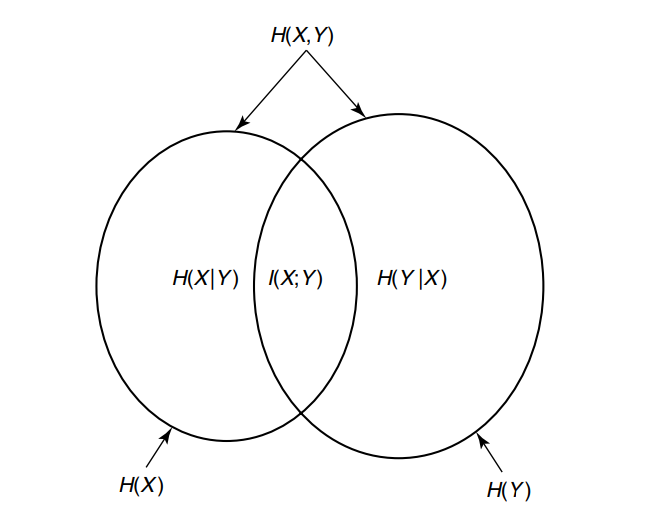
\includegraphics[width=8cm]{img/information_and_entropy.png}
    \caption{Relationship between entropy and mutual information.}
    \label{fig:information_and_entropy}
\end{figure}
Then from the theorem we have also that:
\begin{corollary}[Non negativity of mutual information]
    For any two random variables $X$ and $Y$,
    \begin{equation}
        I(X:Y) \geq 0
    \end{equation}
    with the equality holding iff $X$ and $Y$ are independent. 
\end{corollary}
Another useful result is
\begin{theorem}
    \begin{equation}
        h(X) \leq \log |\alp| \, ,
    \end{equation}
    with the equality holding iff $X$ is uniformly distributed.
\end{theorem}
\begin{proof}
    if $X$ is distributed w.r.t. $\mu$ and if $p(x)= \frac{1}{|\alp|}$ is the uniform distribution,
    \begin{equation*}
        o \leq d(\mu || p) = \sum_{x \in \alp} \mu(x) \log \frac{\mu(x)}{p(x)} = \log |\alp| - h(X) \, .
    \end{equation*}
\end{proof}
And finally from the positivity condition $0 \leq I(X:Y) = h(X) - h(X|Y)$ we have that
\begin{theorem}[Information can't hurt]
    \begin{equation}
        h(X|Y) \leq h(X)
    \end{equation}
    with equality holding iff $X$ and $Y$ are independent.
\end{theorem}
Intuitively, the theorem says that knowing another random variable $Y$ can only reduce the uncertainty in $X$. Note that this is true only on the
average. Specifically, $H (X|Y = y)$ may be greater than or less than or equal to $H (X)$, but on the average $H (X|Y ) =\sum_y p(y)H (X|Y = y) \leq H (X)$. For example, in a court case, specific new evidence might increase uncertainty, but on the average evidence decreases uncertainty.
\\Let's now end this chapter with some last properties of entropy. These come straightforward from the so called \textit{log sum inequality}:
\begin{theorem}[Log sum inequality]
    \begin{equation}
            \sum_{k=1}^n a_k \log \frac{a_k}{b_k} \geq \big( \sum_{k=1}^n a_k \big) \log \frac{\sum_{k=1}^n a_k}{\sum_{k=1}^n b_k}   
    \end{equation}
    with equality holding if and only if $\frac{a_k}{b_k}$ is constant. 
\end{theorem}
There are two consequences of the log sum inequality:
\begin{theorem}
\hfill
    \begin{itemize}
        \item[1)] Convexity of relative entropy:
        \\$d(\mu || \nu)$ is convex in the pair $(\mu, \nu)$, i.e. for any two pairs $(\mu_1, \nu_1)$ and $(\mu_2, \nu_2)$  and $\forall 0 \leq \lambda \leq 1$ we have 
        \begin{equation*}
            d(\lambda \mu_1 + (1 - \lambda) \mu_2 || \lambda \nu_1 + (1 - \lambda) \nu_2 ) \leq \lambda d (\mu_1 || \nu_1) + (1 - \lambda) d (\mu_2 || \nu_2)
        \end{equation*}
        \item[2)] Concavity of entropy:
        \\$h(\mu)$ is a concave function of $\mu$
    \end{itemize}
\end{theorem}
\begin{proof}
    \hfill
    Just apply the log sum inequality y to a single term of the left hand side and then sum over $x \in \alp$:
    \begin{equation*}
        \lambda \mu_1(x) \log \frac{\lambda \mu_1 (x)}{\lambda \nu_1 (x)} + (1 - \lambda) \mu_2(x) \log \frac{(1 - \lambda) \mu_2(x)}{(1 - \lambda) \nu_2(x)}
    \end{equation*}
    Concavity of entropy  follows from the convexity of the relative entropy $d$ and from the relation
    \begin{equation*}
        h(\mu) = \log |\alp| - d (\mu || p) \, ,
    \end{equation*}
    where $p(x)$ denotes the uniform probability distribution.
\end{proof}






